\documentclass[conference]{IEEEtran}
\IEEEoverridecommandlockouts
% The preceding line is only needed to identify funding in the first footnote. If that is unneeded, please comment it out.
\usepackage{cite}
\usepackage{amsmath,amssymb,amsfonts}
\usepackage{algorithmic}
\usepackage{enumitem}
\usepackage{graphicx}
\usepackage{textcomp}
\usepackage{xcolor}
\def\BibTeX{{\rm B\kern-.05em{\sc i\kern-.025em b}\kern-.08em
    T\kern-.1667em\lower.7ex\hbox{E}\kern-.125emX}}
\graphicspath{{Figures/}}

\begin{document}

\title{Secure Industrial Control System with Intrusion Detection\\
% {\footnotesize \textsuperscript{*}Note: Sub-titles are not captured in Xplore and
% should not be used}
}

\author{\IEEEauthorblockN{M Rayhan Ahmed Mithu}
\IEEEauthorblockA{\textit{Computer Science Department} \\
\textit{Tennessee Technological University}\\
Cookeville, TN, United States of America \\
mmithu42@students.tntech.edu}
\and
\IEEEauthorblockN{Michael Rogers, Denis Ulybyshev}
\IEEEauthorblockA{\textit{Computer Science Department, CEROC} \\
\textit{Tennessee Technological University}\\
Cookeville, TN, United States of America \\
mrogers, dulybyshev@tntech.edu}
% \IEEEauthorblockN{3\textsuperscript{rd} Given Name Surname}
% \IEEEauthorblockA{\textit{dept. name of organization (of Aff.)} \\
% \textit{name of organization (of Aff.)}\\
% City, Country \\
% email address}
% \and
% \IEEEauthorblockN{4\textsuperscript{th} Given Name Surname}
% \IEEEauthorblockA{\textit{dept. name of organization (of Aff.)} \\
% \textit{name of organization (of Aff.)}\\
% City, Country \\
% email address}
% \and
% \IEEEauthorblockN{5\textsuperscript{th} Given Name Surname}
% \IEEEauthorblockA{\textit{dept. name of organization (of Aff.)} \\
% \textit{name of organization (of Aff.)}\\
% City, Country \\
% email address}
% \and
% \IEEEauthorblockN{6\textsuperscript{th} Given Name Surname}
% \IEEEauthorblockA{\textit{dept. name of organization (of Aff.)} \\
% \textit{name of organization (of Aff.)}\\
% City, Country \\
% email address}
}

\maketitle

\begin{abstract}
Security breaches in Industrial Control Systems may have a significant impact on human lives and may cause significant financial loss. For that reason, it is important to detect intrusions and anomalies in Industrial Control Systems at early stages to prevent failure developments. Detection of intrusion based on only network data might not be sufficient as sometimes a number of valid commands and events could lead to a critical state. As a result, the number of false positives and false negatives generated by the intrusion detection system rises. In this paper, we propose a novel approach of using device state information, stored in a secure data container, to improve the detection accuracy. Our methodology allows to detect anomalies as well as their root causes.  
To detect a root cause of anomaly, it is essential to provide confidentiality and integrity for log records. In this paper, we also present a secure data container that is used to protect log records as well as state data for devices in cyber-physical systems. Data protection is provided in transit and at rest. Our data container supports role-based and attribute-based access control, so that every party can access only those data subsets for which the party is authorized. Furthermore, we address the insider threat by detecting several types of data leakages that can be made by malicious authorized insiders. 
\end{abstract}

\begin{IEEEkeywords}
intrusion detection, data privacy, industrial control systems, SCADA systems 
\end{IEEEkeywords}

\section{Introduction}
Industrial Control System (ICS) is the technology used to automate the manufacturing process. It is responsible for controlling and managing large number of field devices. The manufacturing industry has seen a huge rise in the adoption of ICS in recent years. The fierce competition among the companies has been the main catalyst for this revolution in the manufacturing industry. According to the study report published by  Market Research Future (MRFR), the industrial control system market will be growing even more in the future \cite{c1}. A lot of these industrial control system are deployed in critical infrastructures such as the smart grid, health care system, water purification, nuclear plants. As a result, any kind of security breach and attack can have significant impact on human lives as well as be very costly. Securing these systems has become a priority as a result of the increasing number of attacks in these domain. 
Even though there are a lot of approaches for intrusion detection in ICS are present in the literature, we observe that most of these solutions focus on the network traffic data generated in the ICS. We propose to use device state information along with network data packets to detect intrusions. If intrusion is detected in a data network on level 2 (see Fig.1), we query device at a lower level 1 to check  device state related to the network data that caused intrusion alert on a higher level. Our approach verifies the alert generated by an Intrusion Detection System (IDS) by validating the suspicious network data packet against the device state information. The algorithm verifies whether suspicious network packet that caused IDS alert is suspicious from the standpoint of a lower level device. This allows not only to detect anomaly, but also to find the root cause of anomaly. Device state data is stored in a secure data container, which guarantees confidentiality and integrity of data that is used to detect anomaly root cause. Secure data container provides data protection in transit and at rest. Data and access control policies are stored in the container in encrypted form. Separate encryption keys, one per data subset, are generated on-the-fly and are not stored neither inside the container nor on any Trusted Third Party (TTP). Data container supports role-based and attribute-based access control, so that every party can access only those data subsets for which the party is authorized. Central Authority (CA) is not required neither for recipient key generation nor for access control policy enforcement, since access control policies are stored inside the container in encrypted form.      
The rest of the paper is organized as follows. Section II presents an overview of related work. Section III <Denis will finish>... 

\section{Related Work}

Concerns over the security of industrial control system has led many researchers to look for different security solutions to protect the network. In this paper we focus on the software solutions that are available in the state of the art. Intrusion detection is one of the most popular techniques used to prevent and detect unauthorized action. The same technique with various approaches are proposed by many researchers to use in the industrial network. 
\par In \cite{c2}, the authors proposed an intrusion detection system that focuses on devices that are connected with serial link. The authors proposed a Snort-based intrusion detection system for MODBUS RTU/ASCII communication. The MODBUS traffic is converted to MODBUS TCP/IP and sent to Snort for rule matching. Snort was implemented in two setup, one was in passive mode where the traffic is only monitored by Snort and in inline setup includes rules for dropping packets.
\par A multi agent intrusion detection system was proposed by Tsan and Kwong \cite{c3} in industrial network. They implemented the unsupervised Ant Colony Clustering Model (ACCM) in the "decision agent" that is responsible for learning and classification of prepossessed data. This implementation shows the improved performance ant-based clustering. The KDD-Cup99 dataset was used for the test evaluation with different clustering algorithms and feature extraction techniques. K-Means clustering achieves 89.17\% average detection rate and  4.29\% false positive rate with the Fast Independent Component Analysis (FastICA) feature extraction.
\par A critical state analysis-based intrusion detection approach by Carcano et al. \cite{c4} in SCADA systems uses state information. In this approach the authors defined a language for system description and to represent states of the system. A software virtual image with software object representing all devices of the monitored system was used to monitor the evolution of system states. Critical states were defined with critical formulas. The intrusion detection system was implemented on the virtual image and if the current state was moving towards a critical state an alert was generated.

\section{Core Design}
% \subsection{Industrial Control Systems Security}
Industrial control system was initially designed to operate within a close environment and manage the overall system. However, this has changed as the ICS network is now globally connected via the internet technology. The global connection has a lot of benefits that includes managing multiple field sites with thousands of devices in different location from one control center, faster data access and and inseparability among devices with different communication protocols. It also exposed the industrial control system to all the vulnerabilities and security threats that exists in the commercial network.Communication among the main components such as programmable logic controller (PLC), supervisory control and data acquisition (SCADA), Control devices is what makes this whole system functional. The communication protocols for these components are not similar to the typical commercial network protocols. Security was not a big concern when these protocols were designed as the system was kept isolated from the outside world. 
\begin{figure}[htbp]
\centering
\centerline{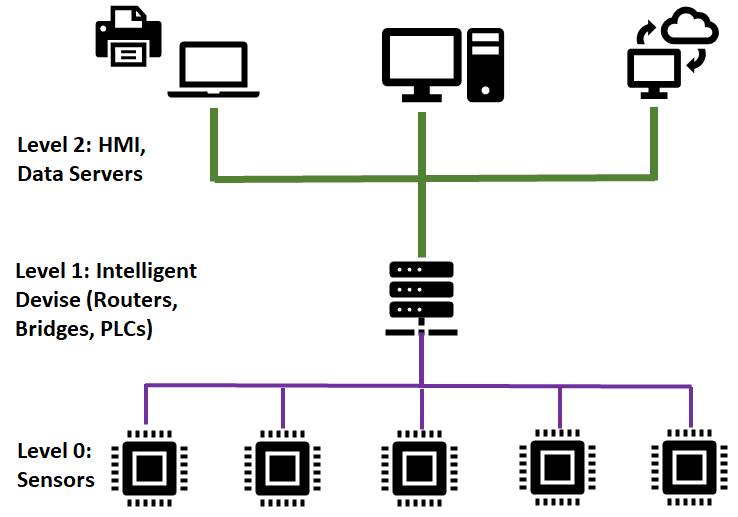
\includegraphics [width=9cm] {ICS-Architecture-RelOK.png}}
\caption{Industrial Control System Architecture}
\label{fig}
\end{figure}
Intrusion detection system is a great method for attack detection and prevention in the commercial network by monitoring network traffic with rule based or anomaly based approach. However, in the industrial network it is not always enough to just monitor the network traffic. It is possible that a sequence of valid commands can lead to a critical situation. As a result, a lot of false positives and false negatives are generated by the IDS. We propose a novel approach where the IDS can validate network traffic with the help from the device generating the traffic. A device state information equivalent to each network packet is created and stored. The device state information is kept in a secure container which can be access upon request. The architecture has three major system components that is focused on completing the steps. Each step will which are:
\begin{enumerate}[label=(\alph*)]
\item Offline Tools for Intrusion Detection
\item SCADA components
\item Secure Container
\item Intrusion Detection Process
\end{enumerate}
\subsection{Offline Tools for Intrusion Detection}
This system component of the architecture is responsible to identify important information about the state of the device and the location of those state information on the device. We call this component the off-line tools as these will be executed when the SCADA system is not running real time. We propose three modules for this component. 
\par The first module is called the \textit{\textbf{Image Mapping Module}}, this module is responsible for identifying the important information to represent the device state and gather those information.
\par The second module will be the \textit{\textbf{Golden Image Module}} which will use the information collected by the image mapping module and create the golden image of the device system which is considered to be safe and standard. \par The third module in this component is the \textit{\textbf{Training Module}}, this module will be used to identify the relationship between a device state and the generated network packet. The training module will be fed data collected from the SCADA environment with different device state and and mapped with the network traffic to automatically link specific network packets to corresponding device state. This information will be provided to the the detection process which can query specific device state information and verify information provided in the network packet to detect intrusion more precisely.

\subsection{SCADA Components}
The second component of our architecture is the SCADA components. This component of the system will monitor system states real time and transfer the state information to the detection process. Two modules are required to execute these actions. The first module is the \textit{\textbf{State Monitor}} and the other module is called \textit{\textbf{State Router}}.
\par The state monitor module is responsible for real time monitoring of the device state. The information collected by the image mapping module in the off-line tools component is used in this module to gather the important sate information from the device. State monitor module will have prior knowledge of what information are necessary to represent the state and where the information are kept in the device. 
\par The device state information collected by the state monitor module will be transferred by the state router module to the node that is computationally more resourceful. This node can perform security analysis to identify if the device is compromised.
\subsection{Secure Data Container}
Proposed solution for protecting data in transit and at rest with providing leakage detection, as well as role-based and attribute-based access control, relies on Secure Mobile Protected Agent with Data (SMPAD). The idea was inspired by an Active Bundle concept [2], [3]. SMPAD is a self-protecting data container that incorporates sensitive data in encrypted form with watermarks, access control policies, metadata, provenance data collector, policy and attribute enforcement kernel. SMPAD can be used to store log files as well as sensor data snapshots. Each separate data subset is encrypted with separate encryption key, generated on-the-fly for each client’s role based on the unique information from the SMPAD execution control flow path. The access control model relies on role-based and attribute-based access control model and guarantees that a client will be able to access only those data subsets from a data container for which the client is authorized [4]. Data container provides tamper-resistance and data integrity. Moreover, SMPAD can detect several types of data leakages that can be made by authorized insiders [1]. The novelty of the proposed solution is that it works in both centralized and decentralized peer-to-peer network architectures. Central Authority (CA) is not required neither for data recipient’s key generation nor for access control policy enforcement.

\begin{figure}[htbp]
\centering
\centerline{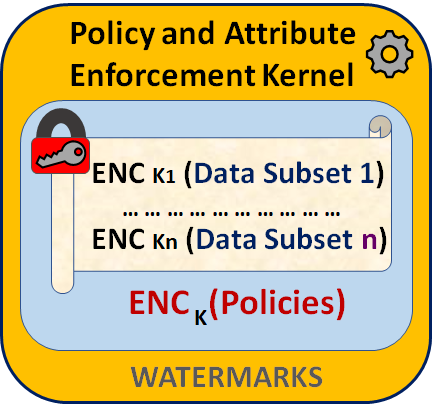
\includegraphics [width=6cm] {SMPAD-RelOK.png}}
\caption{SMPAD: Secure Data Container}
\label{fig}
\end{figure}

%Denis:
- mention difference between SMPAD and EA3B (Exc)
- list set of supported attributes for ABAC
- talk about on-the-fly key generation scheme
- talk about data leakage detection via watermarks

 
\subsection{Intrusion Detection Process}
Detection process is the most important component of the secure architecture. This process is responsible for intrusion detection in the SCADA environment. Typical intrusion detection system (IDS) uses the network packets to analyze the traffic and generate alert in case of any abnormal activity in the network. However, in SCADA environment, it is not necessary that an abnormal network behavior will always be the reason for intrusion. Often times a series of valid commands can lead to a critical situation in the SCADA environment that will cause serious damage to the infrastructure. The IDS will not generate any alert in that situation as the network traffic will not look suspicious or abnormal.
\par The intrusion detection system in this component uses the information gathered by the training module in the off-line tools component to learn about device state. The IDS also receives real time information from the state router and performs analysis to detect compromised device. The information from the state router is also used to improve the IDS detection engine based on the accuracy of intrusion detection. The main idea in the detection process is to provide additional information to the IDS along with the network packets to improve the detection method. The device state information will help the IDS to verify any alert generated from analyzing the network traffic of the SCADA system.  
\begin{figure}[htbp]
\centering
\centerline{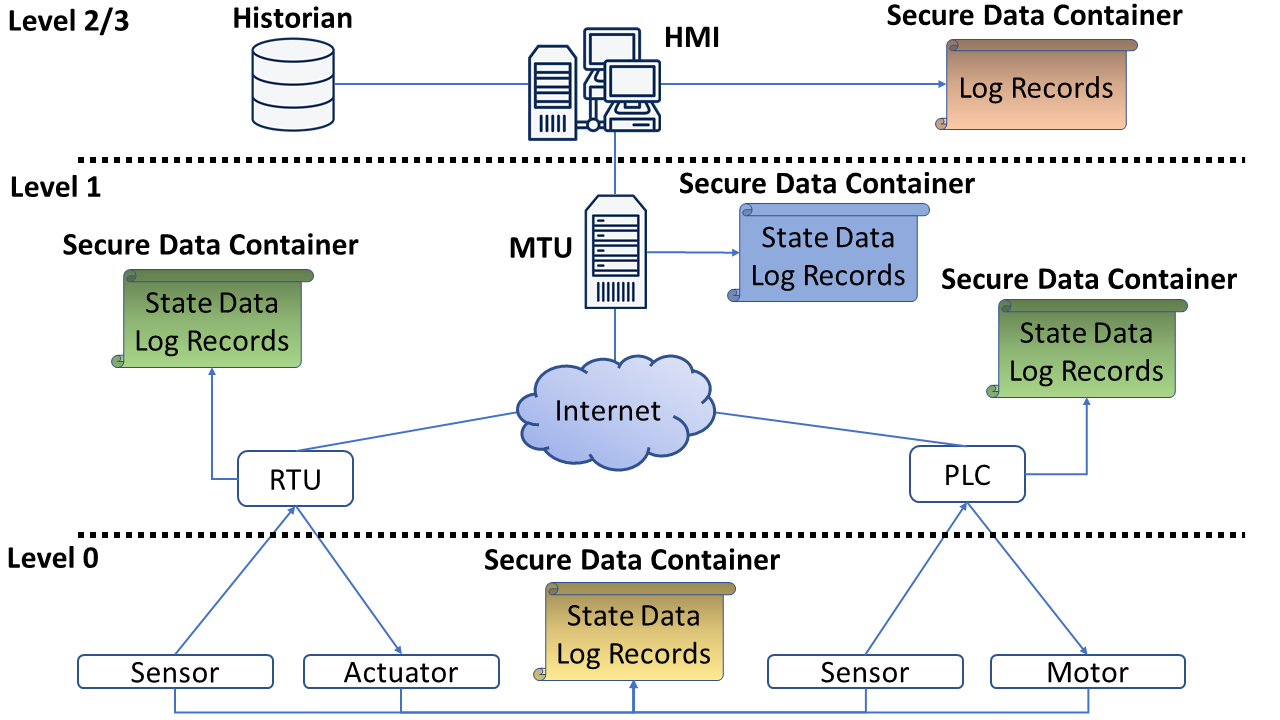
\includegraphics [width=.5\textwidth]{sec_arch.png}}
\caption{Secure Industrial Control System Architecture}
\label{fig}
%
\end{figure}

\section{Evaluation}

\section{Future Work}

\section{Conclusion}




\begin{thebibliography}{00}
\bibitem{c1}Industrial Control Systems (ICS) Market 2018 Global Analysis, Industry Size, Share Leaders, Current Status by Major Key vendors and Trends by Forecast to 2023. https://www.marketwatch.com/press-release/industrial-control-systems-ics-market-2018-global-analysis-industry-size-share-leaders-current-status-by-major-key-vendors-and-trends-by-forecast-to-2023-2018-11-29
\bibitem{c2}Morris, T., Vaughn, R., \& Dandass, Y. (2012). A retrofit network intrusion detection system for MODBUS RTU and ASCII industrial control systems. Proceedings of the Annual Hawaii International Conference on System Sciences, 2338–2345. https://doi.org/10.1109/HICSS.2012.78
\bibitem{c3}Tsang, C. H., \& Kwong, S. (2005). Multi-agent intrusion detection system in industrial network using ant colony clustering approach and unsupervised feature extraction. Proceedings of the IEEE International Conference on Industrial Technology, 2005, 51–56. https://doi.org/10.1109/ICIT.2005.1600609
\bibitem{c4}Carcano, A., Coletta, A., Guglielmi, M., Masera, M., Nai Fovino, I., \& Trombetta, A. (2011). A multidimensional critical state analysis for detecting intrusions in SCADA systems. IEEE Transactions on Industrial Informatics, 7(2), 179–186. https://doi.org/10.1109/TII.2010.2099234
\bibitem{c5}Kiss, I., Genge, B., Haller, P., & Sebestyen, G. (2014). Data clustering-based anomaly detection in industrial control systems. Proceedings - 2014 IEEE 10th International Conference on Intelligent Computer Communication and Processing, ICCP 2014, 275–281. https://doi.org/10.1109/ICCP.2014.6937009
\end{thebibliography}
\vspace{12pt}
\end{document}
